\documentclass{standalone}

\usepackage{pgfplots,tikz,amsmath}
\begin{document}
    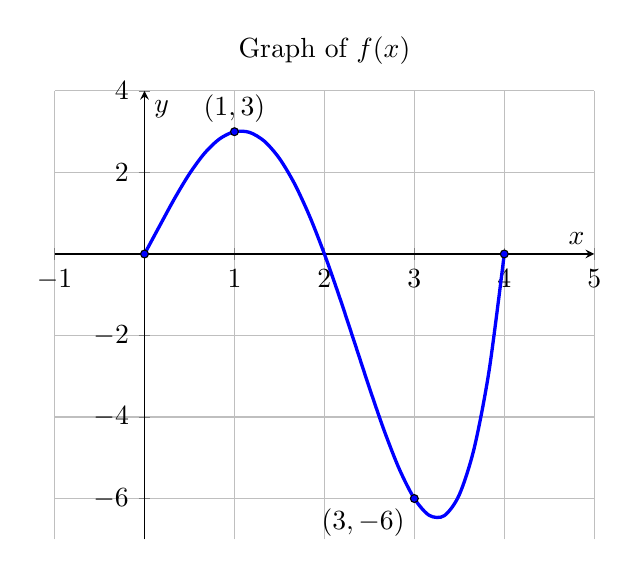
\begin{tikzpicture}
        \begin{axis}[axis lines=center, xmin=-1, xmax=5, ymin=-7, ymax=4, grid,
            xlabel={$x$}, ylabel={$y$}, title={Graph of $f(x)$}]
            \addplot[smooth, blue, very thick, domain=0:4] {0.5*x*(x+1)*(x-2)*(x-4)};
            \draw[fill=blue] (axis cs:0,0) circle(0.05cm);
            \draw[fill=blue] (axis cs:4,0) circle(0.05cm);
            \draw[fill=blue] (axis cs:1,3) circle(0.05cm) node[anchor=south]{$(1,3)$};
            \draw[fill=blue] (axis cs:3,-6) circle(0.05cm) node[anchor=north east]{$(3,-6)$};
        \end{axis}
    \end{tikzpicture}
\end{document}
